
\section{Research Plan}
\label{sec:research-plan}
%include a plan for validation of the research by experimentation and prototyping;

\begin{figure*}[thpb]
      \centering
      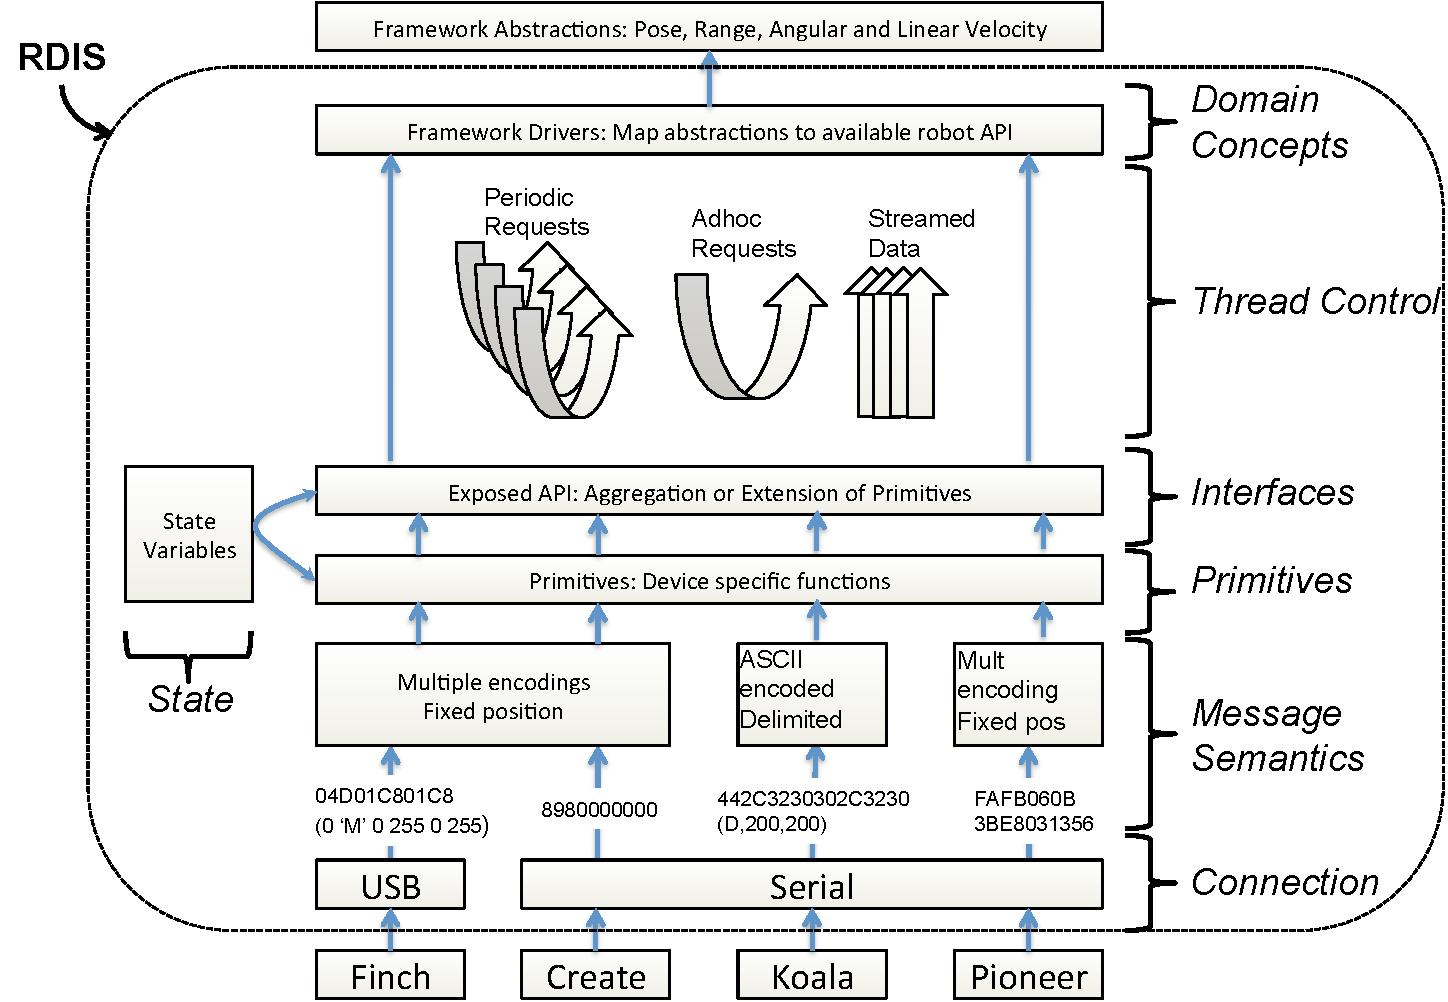
\includegraphics[width=5in]{dm.pdf}
      \caption{Preliminary domain model for mapping devices to frameworks.}
      \label{dm}
\end{figure*}

This preliminary result supports the idea that general robot devices can be described declaratively in a manner that supports discovery and that links to the backend processes.  The RDIS must be expanded to be useful in a larger context.  The work proposed as part of this effort will accomplish the following major innovations to RDIS as a contribution to the engineering of cyber-physical systems: 
\begin{enumerate}
\item Extend the processing models to include a larger set of execution semantics, 
\item Extend the actuation model to include a larger set of popular kinematic chains from both manufacturing and exploration robotics, and
\item Using RDIS as a hardware discovery mechanism, show composition of devices into a controller that is error-aware.   
\end{enumerate}

\subsection{Expansion of execution semantics}

The ability to generalize device to framework mapping requires documenting the concepts in existing mappings.  The domain model captures the invariant features of the device to framework mapping drives the contents of RDIS.  In Figure \ref{dm}, the domain is broken into seven related concepts: 1) connections, 2) state, 3) message semantics, 4) primitives, 5) interfaces, 6) thread control, and 7) robotics domain concepts.  {\sc Connection} refers to the transport used to communicate from the device driver to the framework.  Information needed to establish and maintain the connection is defined within this concept. The {\sc State} definition serves two purposes: 1) define constants relevant to other sections and 2) allow for state to be saved and retrieved as part of adhoc and periodic requests.   The {\sc Message Semantics} refers to the structure of the data which is actually sent to the robot over the connection. This specification is decided by the manufacturer and is generally uniform between primitives.   {\sc Primitives} focuses on describing the firmware interface in order to document the invariant features of the device.   The {\sc Interface} declaration, acting as a logical view of the {\sc Primitives},  specifies functions that are available to a developer to control a robot.   {\sc Domain Concepts} map interfaces to domain specific concepts in a framework agnostic manner.  These concepts are discussed in detail in \cite{Anderson2012}.

\begin{figure*}[thpb]
      \centering
      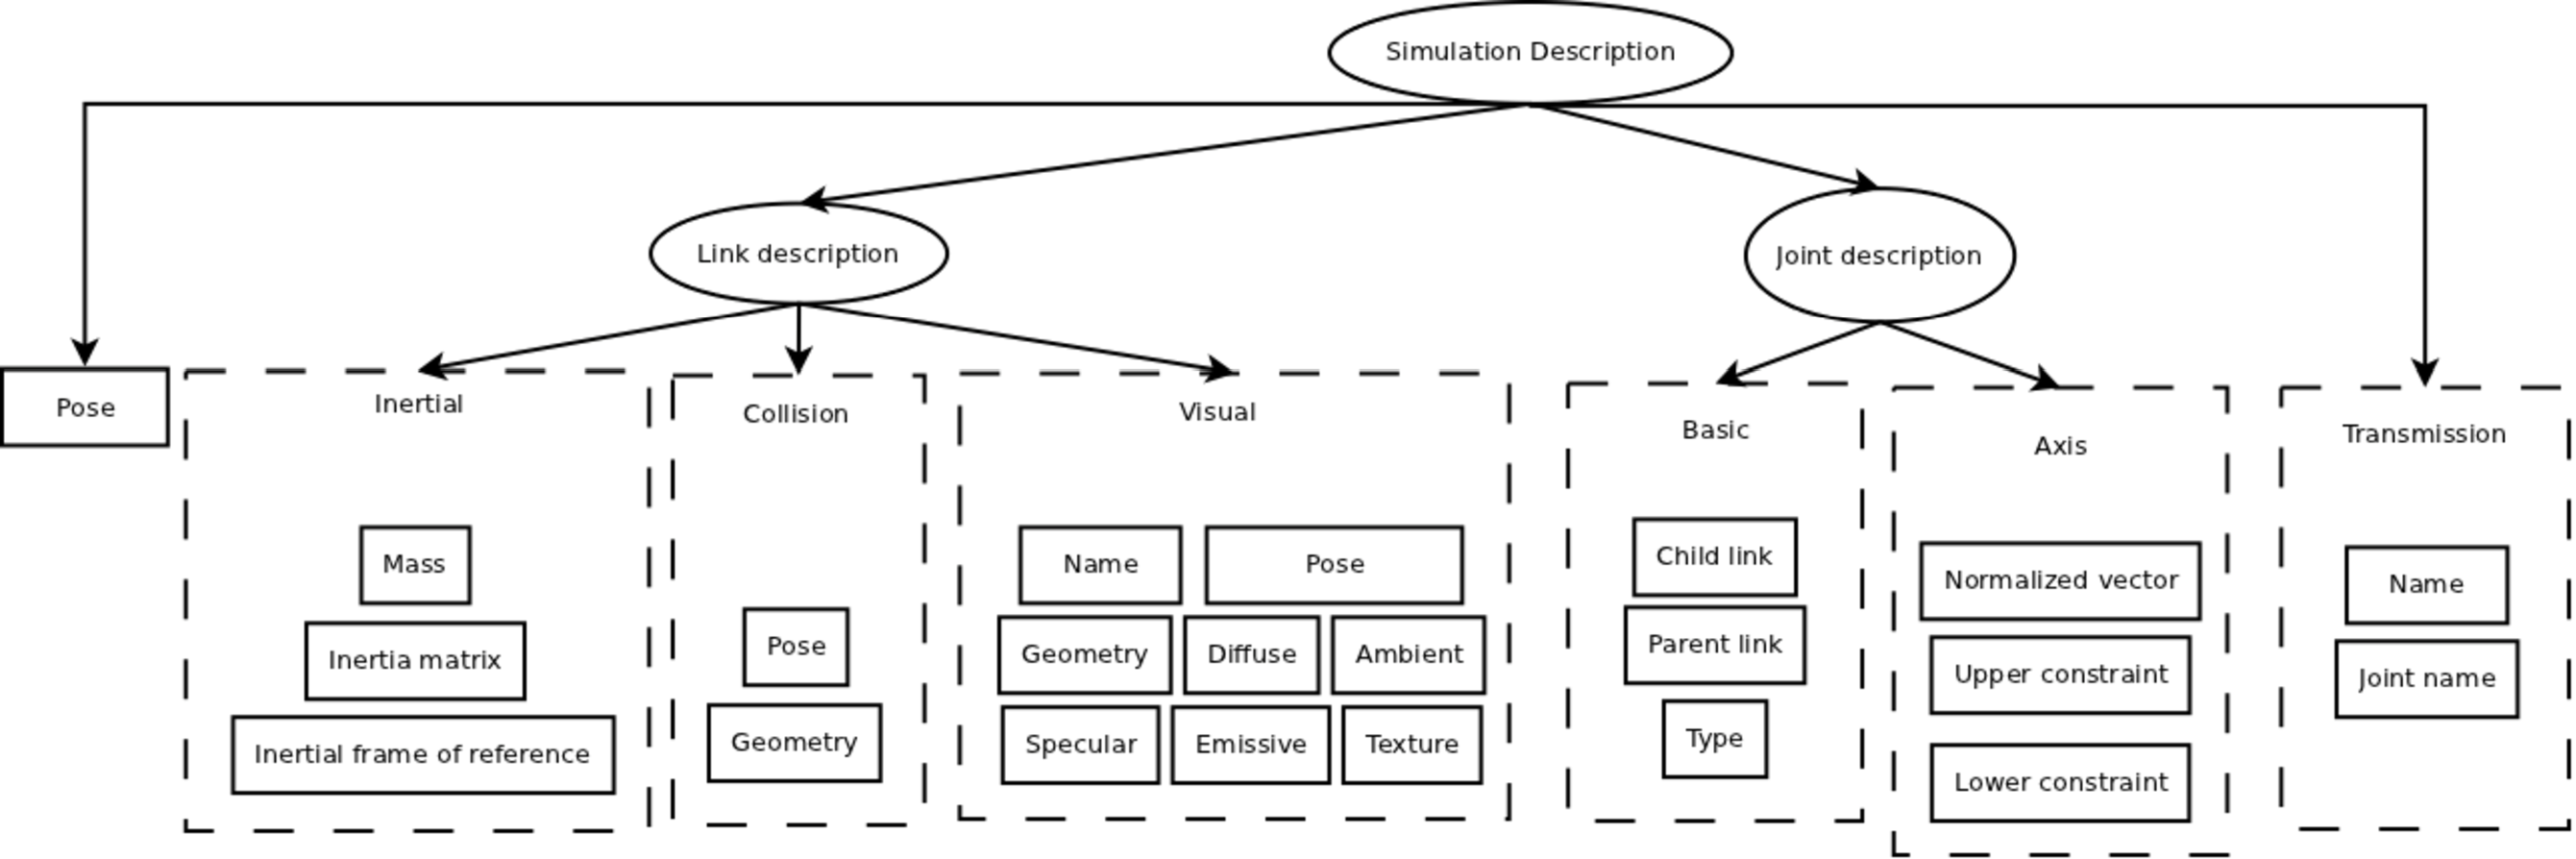
\includegraphics[width=6in]{kvc.pdf}
      \caption{General model for describing kinematics, appearance, collision and dynamics parameters sufficient for simulation on any simulation platform.  Currently targeted platforms include Gazebo, Webots, and ROS.}
      \label{kvc}
\end{figure*}

%These changes require updates to the specification and the underlying set of generation and utilizing tools. 

In this research, we expand the basic implementation of each concept to accommodate a larger set of embedded firmware controllers.  These tasks include: 
\begin{enumerate}
\item Addition of a complete kinematic, visual and collision description consistent with existing simulators and frameworks (see Figure \ref{kvc}).  Although initial focus will be upon the initial kinematic design (differential drive), the proposed model is designed to accommodate other kinematic designs.
\item Standard mechanism for error handling and notification at both the communication and primitive levels.  Error handling examples include re-establishment of connection or actions to take based on output parameters.  This is particularly relevant to platforms that require a heartbeat request periodically.
\item Expansion of the initial single-threaded implementation to include dual and multi-threading models.  A dual model accommodates different input and output threads while a multithreaded model support different frequencies for periodically submitted requests. 
\item Refinement of the state concept and how it matches to primitives and interfaces would provide a scripting language for transformation of data.  The state variable concept is instrumental in implementing periodic requests asynchronously from the client request/reply system.
\item Management of sensor and actuator error models consistent with existing frameworks will allow for manufacturer provided error models to be propagated to the framework or controller.  An example would be a transformation of encoder error to pose error.  Although all sources of error (systematic and non-systematic cannot be accounted for in this approach, it is currently better than existing approaches that abstract out specific device errors.
\end{enumerate}



\subsection{RDIS-enabled tools}
{\bf talk about how we can use rids to assist with development of controller by using existing tools for domain modeling}
